\subsection{Identifying Component 6 in Figure T-2}
\label{T6C06}

\begin{tcolorbox}[colback=gray!10!white,colframe=black!75!black,title=T6C06]
What is component 6 in figure T-2?

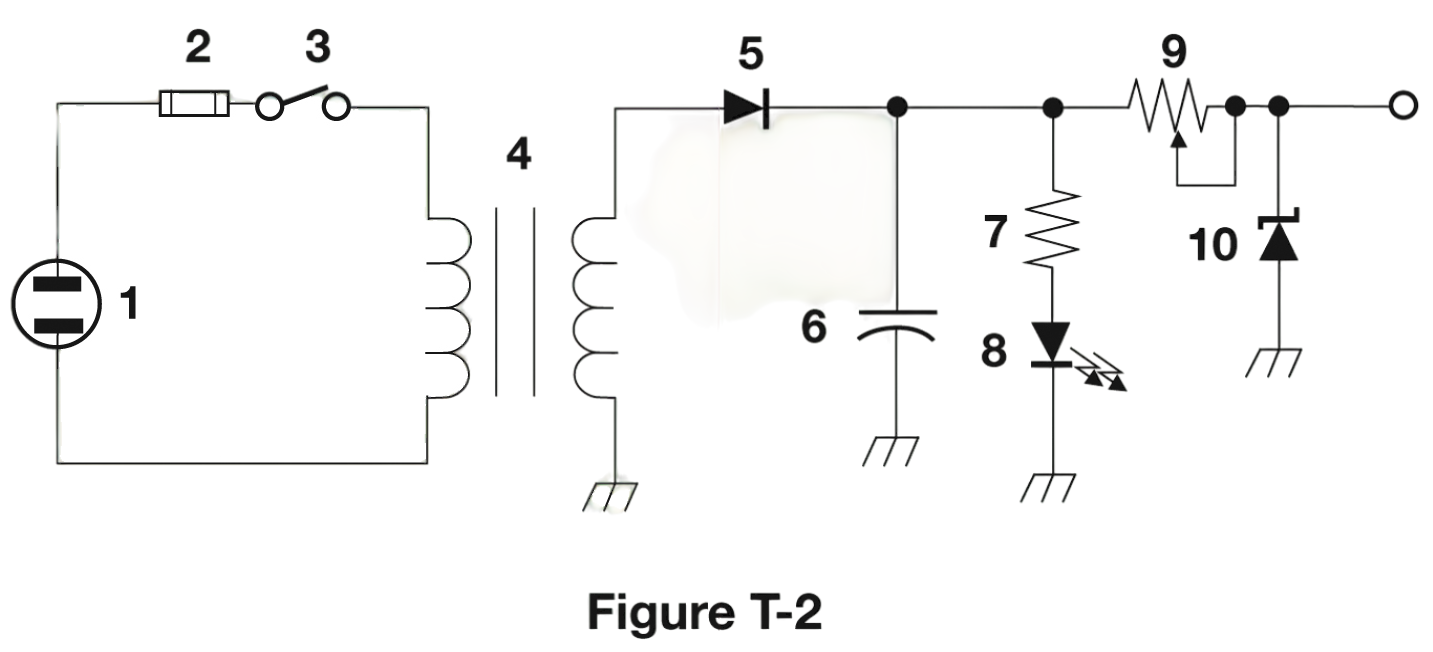
\includegraphics[width=0.5\textwidth]{tech/images/t2.png} 



\begin{enumerate}[label=\Alph*)]
    \item Resistor
    \item \textbf{Capacitor}
    \item Regulator IC
    \item Transistor
\end{enumerate}
\end{tcolorbox}

\subsubsection{Intuitive Explanation}
Imagine you have a water tank with a small hole at the bottom. When you pour water into the tank, it doesn't all flow out immediately; instead, it takes some time. A capacitor is like that water tank but for electricity. It stores electrical energy and releases it slowly. So, when you see component 6 in figure T-2, think of it as the electricity storage tank in the circuit.

\subsubsection{Advanced Explanation}
A capacitor is a passive electronic component that stores electrical energy in an electric field. It consists of two conductive plates separated by an insulating material called a dielectric. The capacitance \( C \) of a capacitor is given by the formula:

\[
C = \frac{Q}{V}
\]

where \( Q \) is the charge stored on one of the plates, and \( V \) is the voltage across the plates. The unit of capacitance is the farad (F). In practical circuits, capacitors are used for filtering, energy storage, and timing applications. In the context of figure T-2, component 6 is identified as a capacitor based on its symbol and role in the circuit.

% Prompt for generating a diagram: A diagram showing the symbol of a capacitor and its placement in a simple circuit would be helpful for visual learners.